%% LyX 2.2.2 created this file.  For more info, see http://www.lyx.org/.
%% Do not edit unless you really know what you are doing.
\documentclass[english]{article}
\usepackage[T1]{fontenc}
\usepackage[latin9]{inputenc}
\usepackage{courier}
\usepackage{gensymb}
\usepackage{graphicx}


\makeatletter

%%%%%%%%%%%%%%%%%%%%%%%%%%%%%% LyX specific LaTeX commands.
%% Because html converters don't know tabularnewline
\providecommand{\tabularnewline}{\\}

\makeatother

\usepackage{babel}
\begin{document}

\title{ARA Smart Power System\\
User Manual}
\maketitle

\section{Introduction}

A photo of the DAQ box component of the power distribution system, with parts labeled, is given in figure \ref{fig:adaq}.

\begin{figure}[h]
\centering
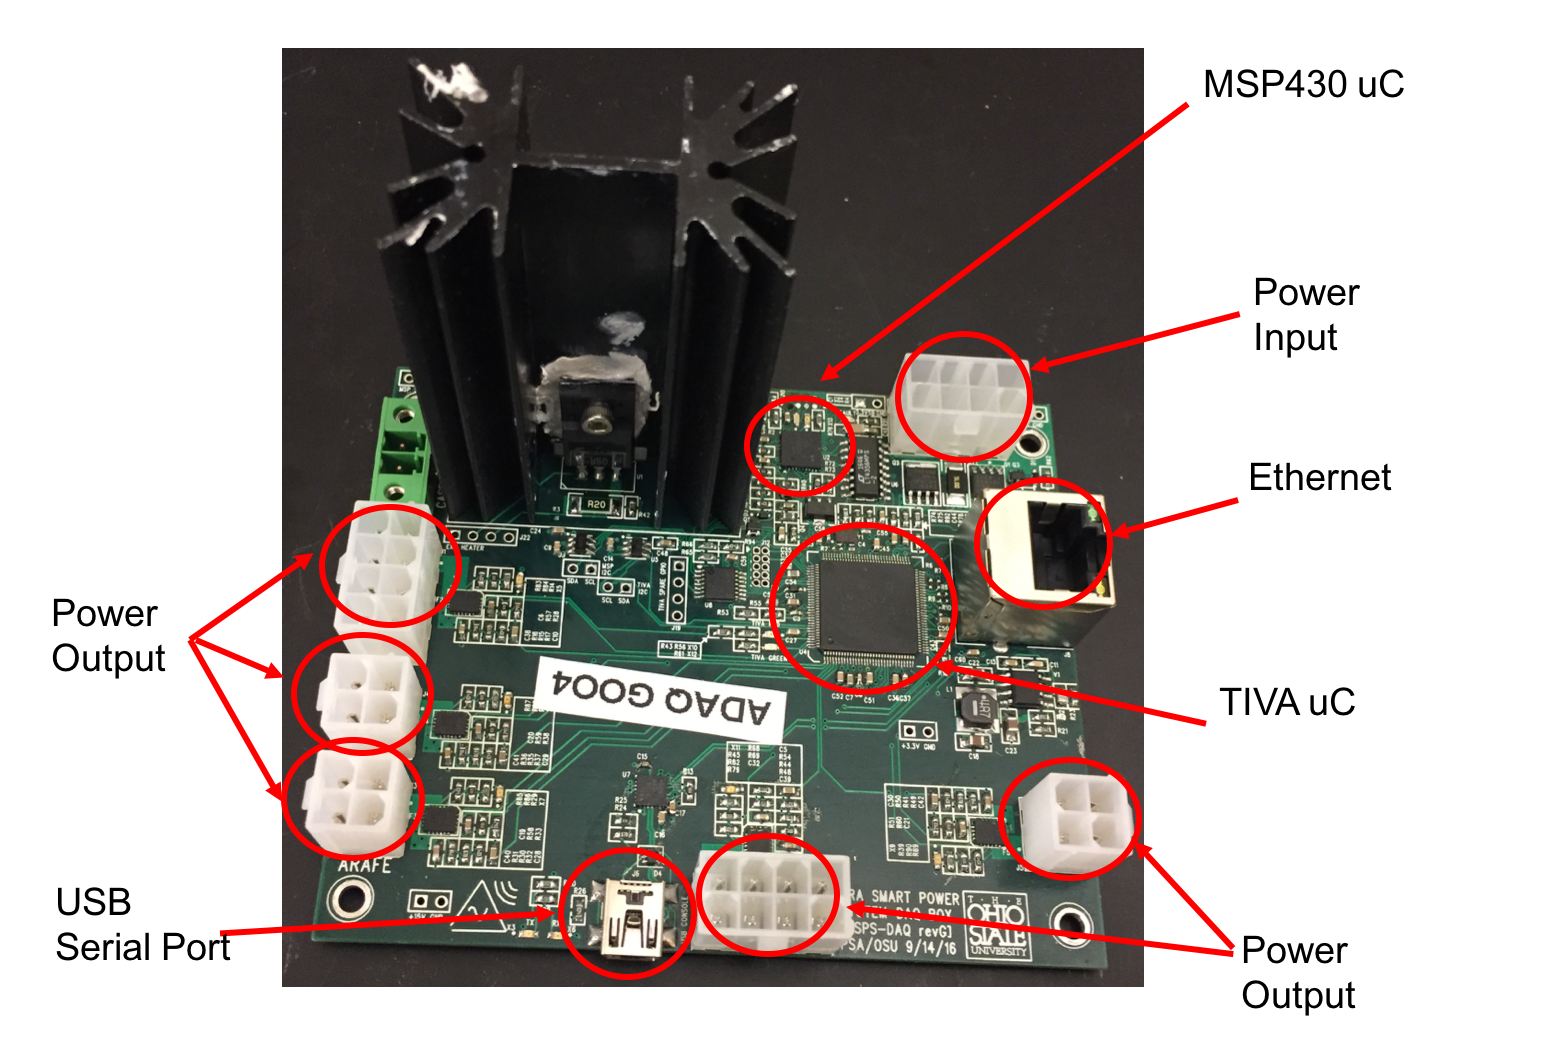
\includegraphics[width=.8\textwidth]{figures/adaq_withnotes.png}
\caption{A picture of the ADAQ (ADAGG004) with major components listed.}
\label{fig:adaq}
\end{figure}

\section{Power Box}

\section{DAQ Box Web Interface}

\subsection{Main control page}

The main ASPS-DAQ microcontroller presents a web page that allows
monitoring/control of all outputs in the DAQ box, with the exception
of the fiber transceiver, for obvious reasons. The fiber transceiver
\emph{can }be disabled through the USB serial command interface.

\subsection{Ethernet Serial Servers}

The main ASPS-DAQ microcontroller presents serial servers on several
ports.
\begin{itemize}
\item Port 23: ASPS-DAQ Heater debug/reprogramming port
\item Port 24: ASPS-Power serial port
\item Port 25: SBC serial port
\item Port 26: ASPS-DAQ Heater command/monitoring interface
\end{itemize}
To access any of these ports simply telnet to them. For example: \texttt{telnet 128.xxx.xxx.xxx 24}

Note, however, that many Telnet clients automatically echo normally,
and so therefore some care is needed to avoid any hassles. In addition,
the Console Redirection in the SBC's BIOS uses VT100-style function
keys, so some configuration is needed.

At the current time, the most appropriate Telnet client for ASPS-DAQ
is PuTTY. In this case, the following options need to be set:
\begin{itemize}
\item Under ``Terminal,'' select ``Force off'' for Local echo.
\item Under ``Keyboard,'' select VT100+ for the Function keys and keypad
setting.
\end{itemize}
With these settings, the complete boot process for the SBC can be
viewed on port 25, and remote BIOS access is possible.

\subsubsection{Resetting serial servers}

Only 1 user can be connected to a serial server at a time. The status
of the serial servers can be seen under the ``serial.html'' page
(e.g. http://ip.address.here/serial.html), and a serial server which
is connected to an unknown client (or a client which failed to close
the connection somehow) can be forcibly disconnected.

\subsection{ASPS-DAQ Heater}

The heater section of ASPS-DAQ serves as a temperature watchdog. At
power on, it holds off activating the remainder of the system until
the temperature has reached a specified target (typically $-40\,\degree \mbox{C}$)
via the use of an onboard adjustable heater. It is the only section
of the ASPS-DAQ board which is required to operate to $-55\,\degree \mbox{C}$.

Communication with the ASPS-DAQ heater is done via a serial connection
through the main ASPS-DAQ microcontroller, which presents it on a
specified TCP port. It should be noted it is \emph{not} possible to
communicate with the ASPS-DAQ heater until the main power has been
activated. Therefore, any changes to the ``autonomous behavior''
parameters should be done with \emph{extreme} caution.

All communication is done via JSON packets.

There is \emph{also} a secondary serial port interface to the main
ASPS-DAQ microcontroller, used for debugging and bootstrap reprogramming.
This is also presented on a specified TCP port. Entering the device
into bootstrap mode is done via the Web interface at http://ip.address.here/bsl.html.

\subsubsection{LED behavior}

\textbf{At power-on, the red LED by the heater will blink 2 times},
indicating power-on cycle behavior. This is a useful thing to note
if seen at any other time, because at power-on, the heater initially
\emph{disables} the main $+15\,\mbox{V}$ rail, which shuts down the
station completely, before running through the decision tree as to
whether or not to power on. (A normal reset does not cause this behavior
- it is only caused by an initial power-on).

At any other time, the red LED indicates that the \emph{PID controller
is working to find the proper current.} The PID controller is extremely
fast, which means that the red LED will only be on briefly once the
current starts to ramp up if the heater is on.

The green LED indicates that the target temperature has been reached
and everything is OK.

\subsubsection{Monitoring}

The ASPS-DAQ heater puts out a constant stream of monitoring data.
Each JSON key contains a specific group of data.

\paragraph{PID data (``pid'' key)}

This key contains an array of (in order) the setpoint, input, and
output of the heater current PID loop. These values are proportional
to the current flowing through the heater. The scale is roughly $1\,\mbox{mA}$
(e.g. $\mbox{setpoint 500}\simeq500\,\mbox{mA}$). 

\paragraph{Temperature data (``temps'' key)}

This key contains an array containing only the local (microcontroller)
temperature at the current moment. Remote temperature will be added
in the future.

\paragraph{Voltage data (``volts'' key)}

This key contains an array containing the input voltage, and the $+15\,\mbox{V}$
voltage. Note that these two should be close to identical if the system
is on.

\subsubsection{Current control}

The setpoint for the heater (which returns to 0 once the system is
above temperature for the wait period) can be modified via a ``current''
key- that is, a JSON packet with a key of ``current'' and a value
equal to the desired setpoint.

\subsubsection{Heater parameters}

The ``autonomous behavior'' parameters can be queried and altered
with the ``heaterparams'' key. Querying is done by sending a JSON
packet with a ``heaterparams'' key and an empty value (or an array
with less than 2 entries). The heater parameters are

\begin{tabular}{|c|c|c|c|}
\hline 
Index & Description & Units & Default\tabularnewline
\hline 
\hline 
0 & Minimum turn-on temperature & $0.01\,\deg\mbox{C}$ & -4000\tabularnewline
\hline 
1 & Heater current when below temp & mA & 500\tabularnewline
\hline 
2 & Maximum wait time below temp & sec & 7200\tabularnewline
\hline 
3 & Wait time after target temp reached & $0.5\,\mbox{sec}$ & 600\tabularnewline
\hline 
4 & P-term in PID & 128 & \tabularnewline
\hline 
5 & I-term in PID & 64 & \tabularnewline
\hline 
6 & D-term in PID & 0 & \tabularnewline
\hline 
\end{tabular}

\emph{Altering} these values is done by sending a JSON packet with
a key of ``heaterparams'', and an array containing the index to
alter (0-6), followed by the new value. Note that changing the P,
I, or D terms could result in very bad behavior, and these changes
are preserved over power cycles!

\section{DAQ Box USB Interface}
In addition to the web interface, the ASPS-DAQ also includes a USB interface, and
can be accessed through the mini-USB port as labeled in figure \ref{fig:adaq}.
It supports 38400/8/N/1 (which is a high baud rate for ARA boards).

One can connect to it with an serial port client, such as TeraTerm, PuTTY, etc.
On a Linux machine, a common way to so would be to use screen,
e.g. \texttt{sudo screen /dev/ttyUSB0 38400}.

After logging in, you will be presented with a user interface as in figure \ref{fig:adaq_interface}.


\begin{figure}[h]
\centering
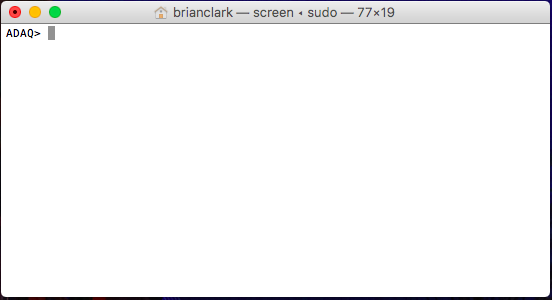
\includegraphics[width=.8\textwidth]{figures/adaq_screen_shot.png}
\caption{A picture of the ADAQ USB interface in a terminal.}
\label{fig:adaq_interface}
\end{figure}

\end{document}
